\documentclass{report}[12pt]
\usepackage{amssymb}
\usepackage{amsmath}
\usepackage{geometry}
\usepackage{cite}
\usepackage[utf8]{inputenc}
\usepackage{graphicx}
\graphicspath{ {images/} }
\usepackage{float}
\usepackage{listings}
\usepackage[dvipsnames]{xcolor}
\usepackage{siunitx}
\usepackage{enumitem}
\usepackage{textcomp}
\usepackage{setspace}
\usepackage{subcaption}


\usepackage{color}   
\usepackage{hyperref}
\hypersetup{
    colorlinks=true, 
    linktoc=all,     
    linkcolor=blue,  
    allcolors=blue
}

\author{Abhishek Rajopaadhye (193230004) \\ Harsha Priyanka Guntaka (193236001) \\ Neelam Patwardhan (193234001)}
\title{Systems and Control Engineering Laboratory (SC 626) \\ Kilobotics}

\begin{document}
\maketitle
\tableofcontents
\listoffigures
\thispagestyle{empty}
\mbox{}

\chapter{Introduction}

\section{Overview}
Kilobots(Figure \ref{fig:Kilobot}) are low cost robots designed at Harvard University's Self-Organizing Systems Research Lab \href{http://www.eecs.harvard.edu/ssr}{http://www.eecs.harvard.edu/ssr}. The robots are designed to make testing collective algorithms on hundreds or thousands of robots accessible to robotics researchers.  

\begin{figure}[H]
	\centering
	\fbox{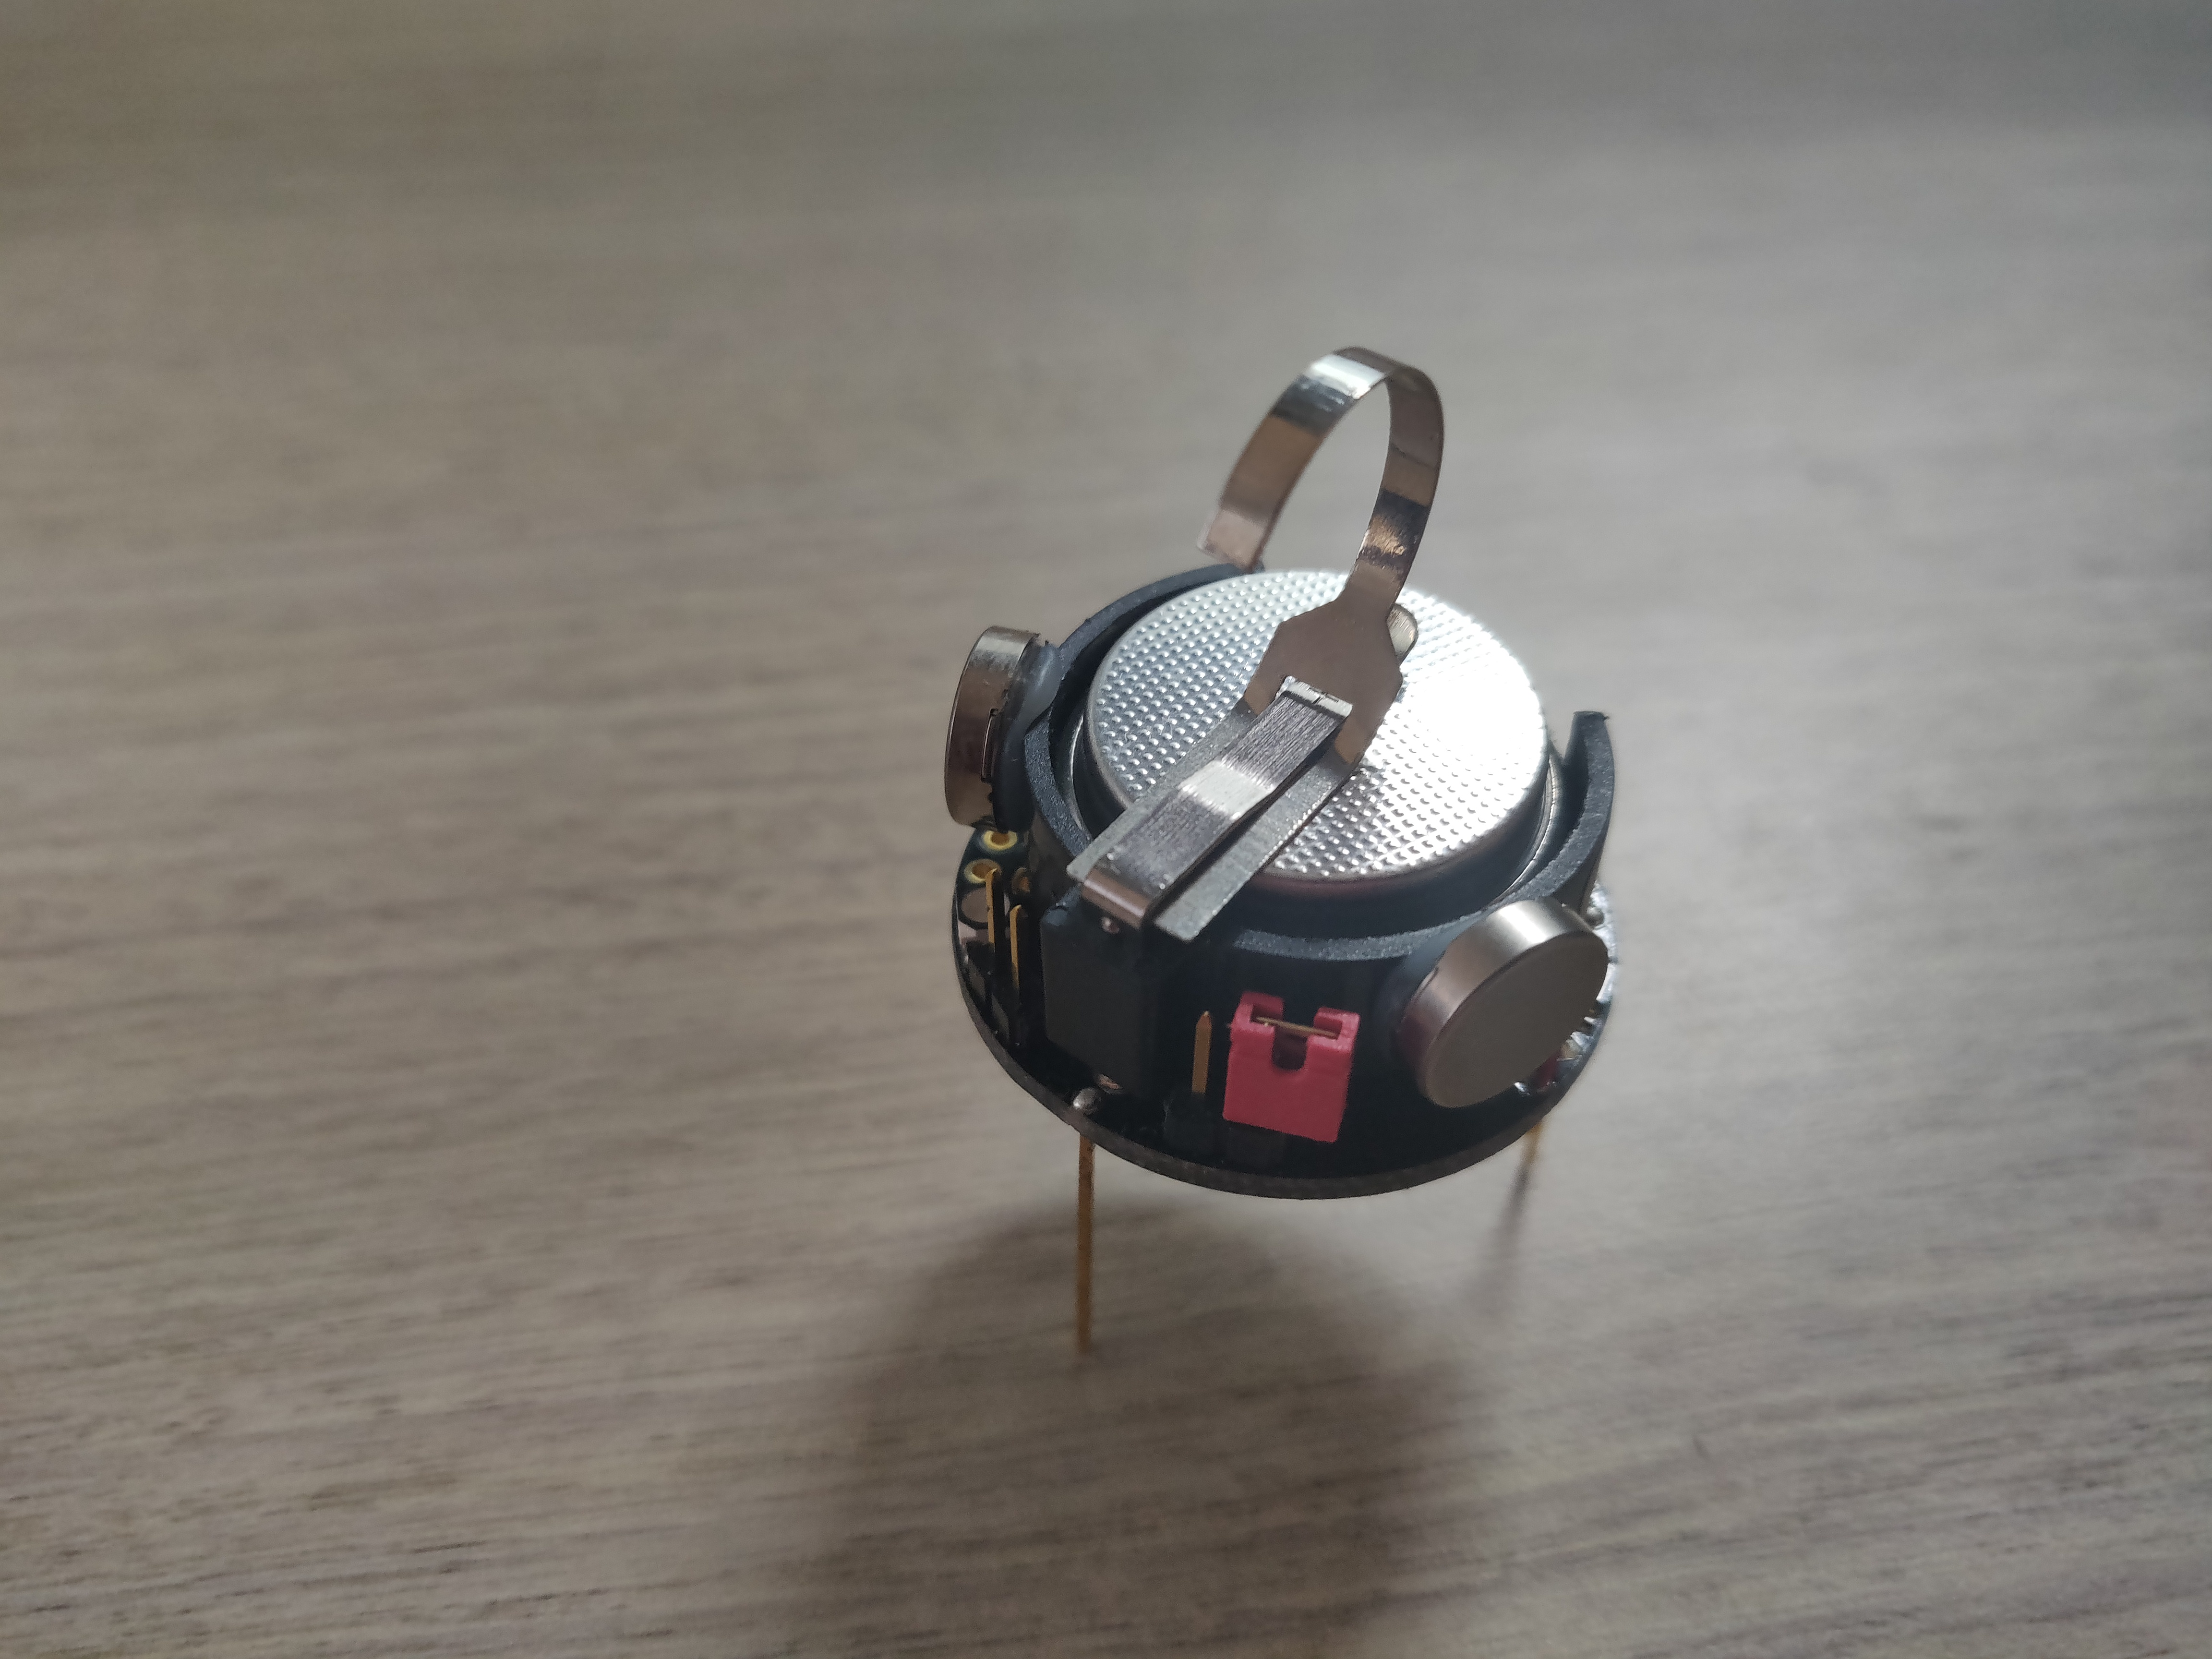
\includegraphics[width=2.5in]{images/kilobot.jpg}}
	\caption{Kilobot}
	\label{fig:Kilobot}
\end{figure}

Though the Kilobots are low-cost, they maintain abilities  similar  to  other  collective  robots. These  abilities  include differential drive locomotion, on-board computation power, neighbor-to-neighbor communication, neighbor-to  neighbor distance sensing, and ambient light sensing. Additionally they are designed to operate such that no robot requires any individual attention by a human operator. This makes controlling a group of Kilobots easy, whether there are 10 or 1000 in the group.

\section{Features of Kilobot}
\begin{itemize}
    \item Processor : ATmega 328p (8bit @ 8MHz) 
    \item Memory : 
    \begin{itemize}
        \item 32 KB Flash used for both user program and bootloader 
        \item 1KB EEPROM for storing calibration values and  other non-volatile data and 2KB SRAM.
    \end{itemize}
    \item Battery : Rechargeable Li-Ion  3.7V, for a 3 months autonomy in sleep mode. Each Kilobot has a built-in charger circuit, which charges the onboard battery when +6 volts is applied to any of the legs, and GND is applied to the charging tab. 
    \item Charging : Kilobot charger for 10 robots simultaneously (optional).
    \item Communication : Kilobots can communicate with neighbors up to 7 cm away by reflecting infrared (IR) light off the ground surface.(Figure \ref{fig:IR sensing})
    \item Sensing : 1 IR and 1 light intensity.
    \begin{itemize}
        \item When  receiving a message, distance to the  transmitting Kilobot can be determined using received   signal strength. The distance depends on the surface  used as the light intensity is used to compute the value.
        \item The brightness of the ambient light shining on a Kilobot can be detected. 
        \item A Kilobot can sense its own battery voltage.  
    \end{itemize}
    \item Movement :  Each Kilobot has 2 vibration motors,    which are independently controllable, allowing for differential drive of the robot. Each motor can be set to  255 different power levels.
    \item Light : Each Kilobot has a red/green/blue (RGB) LED  pointed upward, and each color has 3 levels of brightness control. 
    \item Software : The Kilobot Controller  software (kiloGUI) is available for controlling the controller  board, sending  program files to the robots and controlling them. 
    \item Programming : For programming, the open source  development software WinAVR combined with Eclipse gives a C programming environment. An API with basic functions  such as motor speed, led control, distance measurement is available and some examples are provided.
    \item Dimensions : diameter: 33 mm, height 34 mm (including the legs, without recharge antenna). 
\end{itemize}

\section{Requirements}
\begin{itemize}
    \item Hardware :
    \begin{itemize}
        \item Computer with Microsoft Windows and an USB port (not included)
        \item Kilobot robot 
        \item Over-head controller (OHC) 
        \item Kilobot charger 
    \end{itemize}
    \item Software : To start programming the Kilobot with the new version from kilobotics, we have two solutions. 
    \begin{itemize}
        \item Online editor \url{https://www.kilobotics.com/editor}
        \item  Install WinAVR and Eclipse to compile the whole library on your computer
        \url{https://github.com/mgauci/kilobot\_notes/blob/master/eclipse\_winavr\_setup/eclipse\_winavr\_setup.md}
    \end{itemize}
\end{itemize}

\begin{figure}[H]
	\centering
	\fbox{\includegraphics[width=2.5in]{images/IR-communication.jpg}}
	\caption{IR sensing}
	\label{fig:IR sensing}
\end{figure}


\section{Over-Head Controller(OHC)}
In case of Kilobots, instead of plugging in a charging cable for each robot in order to update its program, each can receive a program via an IR communication channel. This allows an over head IR transmitter to program all the robots in the collective in a fixed amount of time, independent of the number of robots.

\begin{figure}[H]
\centering
	\begin{minipage}{.4\textwidth}
	\centering
	\includegraphics[width=2.0in]{images/OHC.jpg}
	\end{minipage}
	\begin{minipage}{.4\textwidth}
	\centering
	\includegraphics[width=2.0in]{images/programming-OHC.jpg}
	\end{minipage}
\caption{Overhead Controller}
\label{fig:Overhead Controller}
\end{figure}

\section{Motor Calibration}
Kilobot should be operated on a smooth, flat surface to ensure proper robot mobility. Only one Kilobot can be calibrated at the same time. 
\begin{enumerate}
    \item Place the Kilobot in PAUSE mode.
    \item Open KiloGUI interface and then open Calibration mode.(Figure 1.4)
    \item The first line (Unique ID) can be used to save an ID in your Kilobot. This can be useful if you want to save all calibration value for each Kilobot. 
    \item The second line (Turn Left) will configure the kilo\_turn\_left parameter to set the CCW movement. Set  a  value for the motor (approximately 70) and press the Test  button. Adjust the value to obtain a smooth move. 
    \item Do the same as explain in point 4, for the right motor (Turn Right line). 
    \item Next is to set the straight move parameters. Start with the same value for the left and right motor  (approximately 60) and press the Test button. Now adjust the two value to move the Kilobot as straight as possible. 
    \item Finally, when all the parameters are fine, you can press the Save button to write the parameters in the EEPROM of the Robot.
\end{enumerate}

\begin{figure}[H]
\centering
	\begin{minipage}{.4\textwidth}
	\centering
	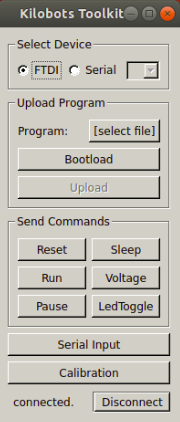
\includegraphics[width=1.5in]{images/kilogui.png}
	\end{minipage}
	\begin{minipage}{.4\textwidth}
	\centering
	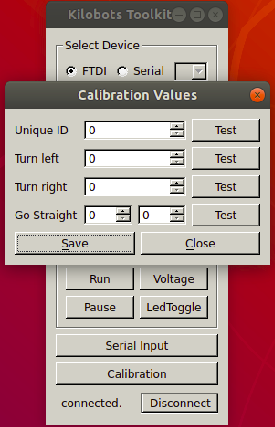
\includegraphics[width=2.2in]{images/kilogui-motor-calib.png}
	\end{minipage}
\caption{Motor calibration using KiloGUI}
\label{fig:Motor calibration using KiloGUI}
\end{figure}

\chapter{Orbiting of Kilobots}

\section{Objective}
Our objective is to make a Kilobot(planet) orbit around 
\begin{itemize}
    \item one stationary Kilobot(star)
    \item multiple stationary Kilobots.
\end{itemize} 

\begin{figure}[H]
	\centering
	\fbox{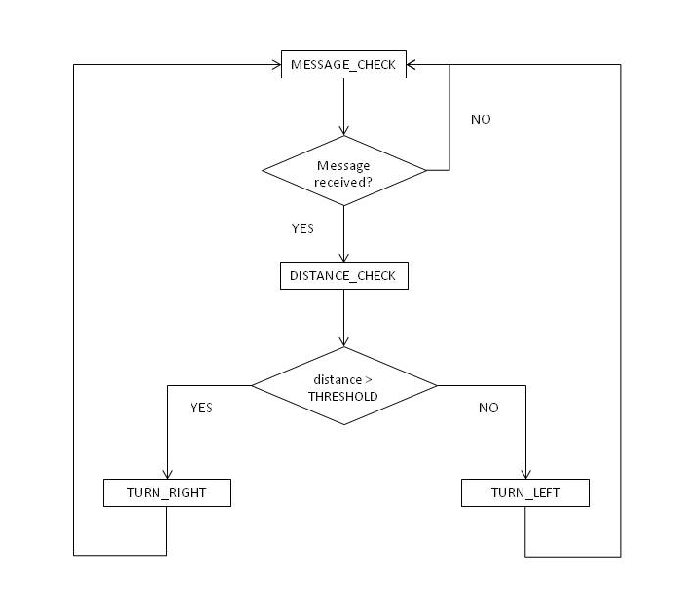
\includegraphics[width=4in]{images/flowchart-planet-star.png}}
	\caption{Flowchart for orbiting a Kilobot(Single star)}
	\label{fig:Flowchart_for_orbiting_a_Kilobot(Single_star)}
\end{figure}

\section{With single stationary Kilobot}
The algorithm for the planet motion with a single star is as follows:
\begin{enumerate}
    \item Check for the message signal from star Kilobot.
    \item If message not received go to step 1.
    \item If message is received, calculate the distance.
    \item If the distance is greater than Threshold value(fixed radius), move right. Else, move left.
    \item Go to step 1.
\end{enumerate}

Flowchart to the corresponding algorithm is illustrated in Figure \ref{fig:Flowchart_for_orbiting_a_Kilobot(Single_star)}.

\subsection{Results and Demonstration}
As per the Kilobotics manual, the maximum and minimum communication ranges are 110mm and 33mm respectively. So we have taken the orbit radius ({\it THRESHOLD}) as 50mm, which falls within good communication range. Also, we have given motor nn time ({\it MOTOR\_ON\_DURATION}) as 500ms.

Video of working demo of problem statement can be accessed from the link in Figure \ref{fig:planet-star-demo}.

\begin{figure}[H]
	\centering
	\fbox{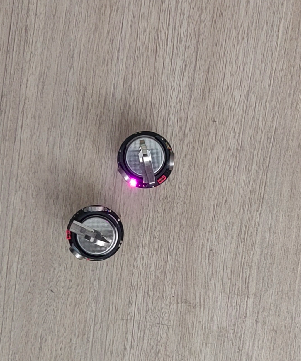
\includegraphics[width=2.5in]{images/planet-star-demo.png}}
	\caption{\href{https://drive.google.com/open?id=1j-bFCbUoinQfT9sqNYdseDKCSMbgUR3y}{Orbiting of Kilobot (Single Star)}}
	\label{fig:planet-star-demo}
\end{figure}

\section{With multiple stationary Kilobots}
We have placed one more Kilobot within the communication range of the planet and star. It was observed that the planet collides with one of the star due to communication delay between them.

Video of working demo can be accessed from the link in Figure \ref{fig:planet-star-collision}.

\begin{figure}[H]
	\centering
	\fbox{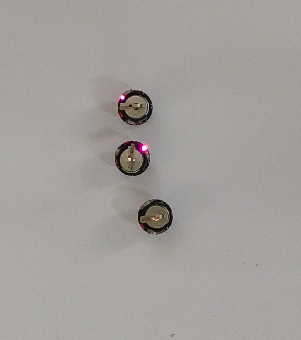
\includegraphics[width=2.5in]{images/planet-mstar-demo.png}}
	\caption{\href{https://drive.google.com/open?id=1gF9iI-mOKVoa7VgCKw3sjqGuXj6nrcXy}{Planet colliding with one of the stars}}
	\label{fig:planet-star-collision}
\end{figure}

To avoid collision, we have modified the above algorithm by checking the message from the neighbor Kilobots for multiple times. The algorithm is as follows:

\begin{enumerate}
    \item First initialize a variable ({\it distance}) corresponding to distance between star and planet to 1000 (or to any other value which is greater than the range of Kilobots).
    \item Check for message from neighbor Kilobots. If you receive the message, estimate the distance, then compare it with the value in the {\it distance} variable and replace the variable with the lowest value.
    \item Go to step 2, until the number of messages received are equal to {\it TOTAL\_NUM\_COMMUNICATION}. 
    \item Now, the value of {\it distance} variable will be our distance between star and planet. If the distance is greater than required orbit radius ({\it THRESHOLD}) move right. Else, move left.
    \item Go to step 1.
\end{enumerate}

The flowchart for the corresponding algorithm is illustrated in Figure \ref{fig:Flowchart_for_orbiting_a_Kilobot(Multiple_star)}.

\begin{figure}[H]
	\centering
	\fbox{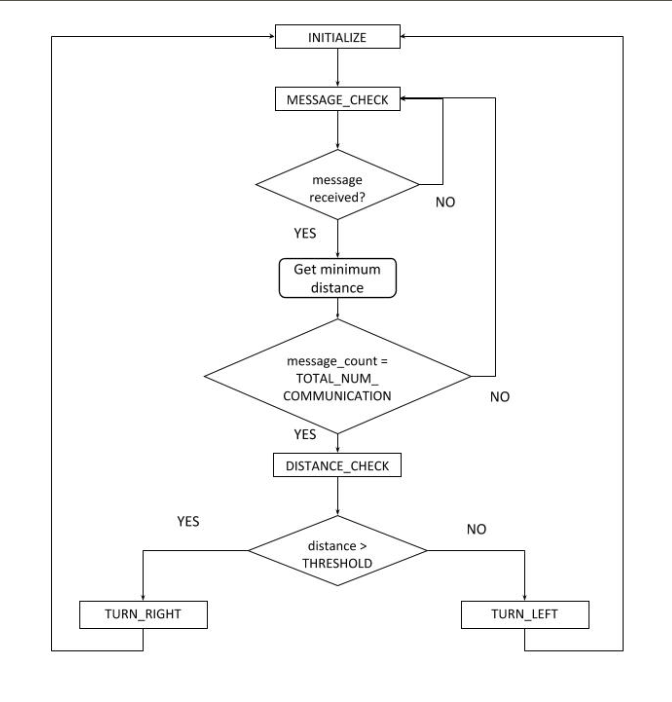
\includegraphics[width=5in]{images/flowchart-planet-mstar.png}}
	\caption{Flowchart for orbiting a Kilobot(Multiple star)}
	\label{fig:Flowchart_for_orbiting_a_Kilobot(Multiple_star)}
\end{figure}

\subsection{Results and Demonstration}
We have used the same orbit radius ({\it THRESHOLD = 50}), and same motor on time ({\it MOTOR\_ON\_DURATION = 500}) as in the case of single star. To avoid collision between Kilobots we have checked for the message for multiple times i.e. {\it TOTAL\_NUM\_COMMUNICATION = 4}.

Video of working demo for this problem statement can be accessed from the link in Figure \ref{fig:planet-mstar-demo-1}.
\begin{figure}[H]
	\centering
	\fbox{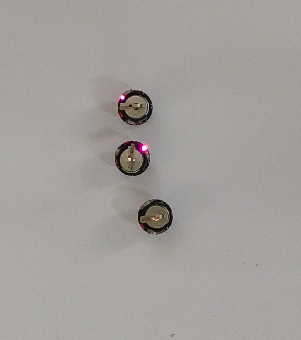
\includegraphics[width=2.5in]{images/planet-mstar-demo.png}}
	\caption{\href{https://drive.google.com/open?id=1LtyCuED4pWMkUGRsmc1yqm-90bjDEhDx}{Orbiting of Kilobot (Multiple Star, {\it MOTOR\_ON\_DURATION = 500}, {\it TOTAL\_NUM\_COMMUNICATION = 4})}}
	\label{fig:planet-mstar-demo-1}
\end{figure}

It can be observed that in this case the speed of the planet Kilobot is less compared to the case with single stationary Kilobot. It can be increased by increasing the {\it MOTOR\_ON\_DURATION} and decreasing the {\it TOTAL\_NUM\_COMMUNICATION}.

Video of working demo for this problem statement can be accessed from the link in Figure \ref{fig:planet-mstar-demo-2}.

\begin{figure}[H]
	\centering
	\fbox{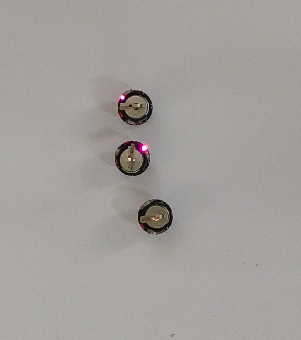
\includegraphics[width=2.3in]{images/planet-mstar-demo.png}}
	\caption{\href{https://drive.google.com/open?id=1f9FGpkbiLwUOuI4cfdkbgaj63m5EHV17}{Orbiting of Kilobot (Multiple Star, {\it MOTOR\_ON\_DURATION = 800}, {\it TOTAL\_NUM\_COMMUNICATION = 3})}}
	\label{fig:planet-mstar-demo-2}
\end{figure}

\chapter{Gradient Formation}
\section{Objective}
Our objective of this experiment to assign unique ids to kilobots using a reference robot. They will get numbered as per their distance from reference robot. This is how the gradient is formed.
\begin{enumerate}
    \item First, we initialize the reference kilobot to 0. This kilobot is going to send the message.
    \item The id's of the other kilobots are assigned based on the distance threshold.
    \item The bot(s) nearest to the reference bot will receive the message and get id 1.
    \item The self unique id of all the other kilobots is preset at 251.
    \item These bots send data and those within the zone of communication with threshold set as 50mm;their unique ids will be checked and updated to +1.If not, the message is checked again.
    \item If there are multiple kilobots within the same zone of communication and falling within the same threshold limit,the one(s) having the least distance are again checked for their id's.
    \item The temporary id is compared to the present self unique id and the one with the least id is updated as the new id of the kilobot(s).
    \item To distinguish between set of kilobots having same id's,they are represented with colors red,blue,green etc.
\end{enumerate}

Flowchart to the corresponding algorithm is illustrated in Figure \ref{fig:flowchart-gradient}.
\begin{figure}[H]
	\centering
	\fbox{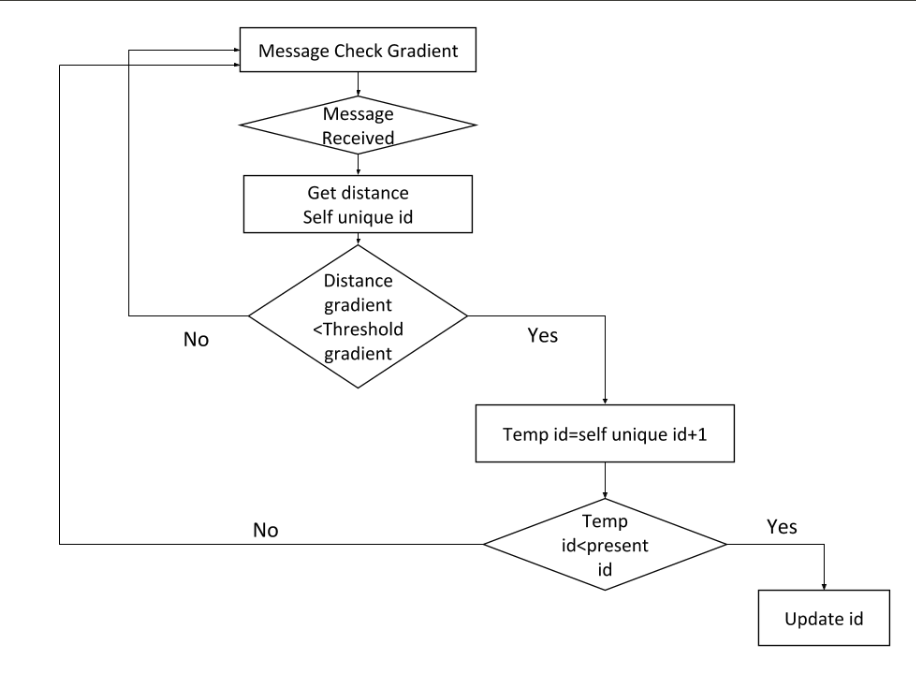
\includegraphics[scale=0.4]{flowchart-gradient.png}}
	\caption{Flowchart for gradient formation}
	\label{fig:flowchart-gradient}
\end{figure}

\section{Results and Demonstration}
To differentiate between different ids of the kilobots they are converted into binary to represent three colors red, blue and green. 
Video of working demo of problem statement can be accessed from the link in Figure \ref{fig:gradient-color}.

\begin{figure}[H]
	\centering
	\fbox{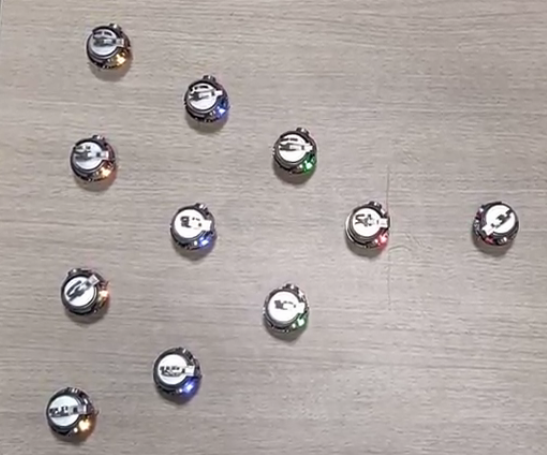
\includegraphics[width=2in]{gradient.png}}
	\caption{\href{https://drive.google.com/drive/folders/14PzarH4uEqTsYBiknOU7pAX3xXhWmLxa}{Display of colors as per different ids}}
	\label{fig:gradient-color}
\end{figure}

\chapter{Edge following}

\section{Objective}
Our objective is to make the kilobots which are on the outer edge to move along the edge of a group of kilobots by measuring distances without being physically blocked and reach the reference bot. 

\begin{figure}[H]
	\centering
	\fbox{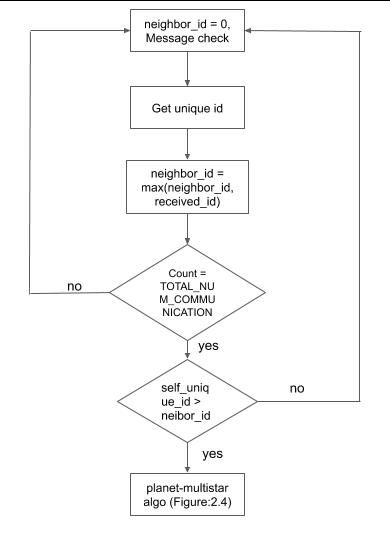
\includegraphics[scale=0.5]{flowchart-edge-following.png}}
	\caption{Flowchart for Edge following}
	\label{fig:Flowchart for Edge following}
\end{figure}

The algorithm is as follows:
\begin{enumerate}
    \item Check for the message from neighboring kilobots for TOTAL\_NUM\_COMMMUNICATION times.
    \item For each message received get the unique id and store the maximum id.
    \item Compare it's own unique id with maximum neighbor id.
    \item If self unique id $>$ max. neighbor id, start moving towards the reference bot using {\textit{planet multistar}} algorithm.
    \item If not, go to step 1.
\end{enumerate}
Flowchart to the corresponding algorithm is illustrated in Figure \ref{fig:Flowchart for Edge following}.

\section{Result and Demonstration}
Kilobots along the outer edge of the initial group are able to move without being physically blocked. They can determine that they are on the outer edge by comparing their gradient values to those of their neighbors. We have used TOTAL\_NUM\_COMMUNICATION=5, so that robot receives enough communication messages from neighbouring bots to identify the position. These robots can then use edge-following around the stationary initial group to reach the reference kilobot. We have used TOTAL\_NUM\_COMMUNICATION\_ORBIT=3, to make sure bot receives right information about distance while orbiting.
Video of working demo of problem statement can be accessed from the link in Figure \ref{fig:Edge Following}.

\begin{figure}[H]
	\centering
	\fbox{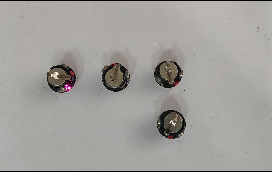
\includegraphics[width=2.5in]{edge-following.png}}
	\caption{\href{https://drive.google.com/file/d/13Svhl9CzhrJuGXXccM-IlZTrmvq1gzwJ/view}{Edge Following with TOTAL\_NUM\_COMMUNICATION=5 and TOTAL\_NUM\_COMMUNICATION\_ORBIT=3}}
	\label{fig:Edge Following}
\end{figure}

It can be observed that once the outer edge (with max. unique id) kilobot goes out of communication range of the next outer edge kilobot, it will start moving towards the reference bot.

\chapter{Gradient formation and edge following integration}

\section{Objective}
Our objective of this experiment is to form gradient with respect to reference robot first and then bring the farthest robot near the reference robot by using edge following algorithm. We are integrating the gradient formation and edge following experiments performed earlier.

The algorithm is as follows:
\begin{enumerate}
    \item We are starting with {\textit{gradient formation algorithm}} as shown in figure 3.1
    \item To make sure that the gradient is stabilized, we have added one more variable called 'count' which will run the {\textit{gradient formation algorithm}} 20 times.
    \item check count $\leq$ TOTAL\_NUM\_COMMUNICATION\_GRADIENT.
    \item If the condition is satisfied then increase the count and run the further loop.
    \item When the count is more than TOTAL\_NUM\_COMMUNICATION\_GRADIENT, then start {\textit{edge following algorithm}} as shown in figure 4.1
\end{enumerate}
Flowchart to the corresponding algorithm is illustrated in Figure \ref{fig:Flowchart for integration of gradient formation and Edge following}.

\begin{figure}[H]
	\centering
	\fbox{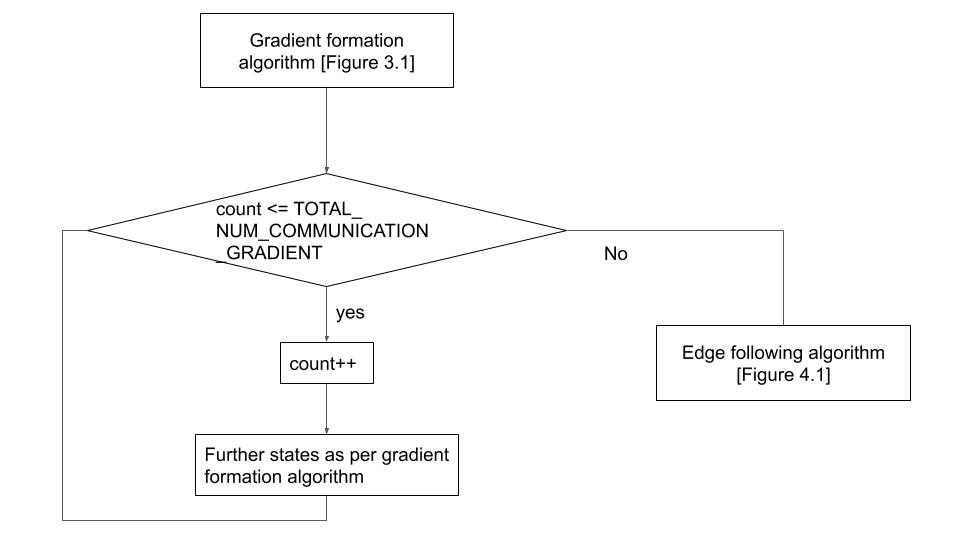
\includegraphics[scale=0.45]{flowchart-gradient&edge-following.jpg}}
	\caption{Integration of gradient formation and Edge following}
	\label{fig:Flowchart for integration of gradient formation and Edge following}
\end{figure}

\section{Result and Demonstration}
We have arranged the robots in one line. When the code is run, firstly the robots are forming gradient which is visible from the LED color. We have kept TOTAL\_NUM\_COMMUNICATION\_GRADIENT = 20 to stabilize the gradient. Then the farthest kilobot starts orbiting, and following the edge of the remaining robots, it comes near the reference robot. We kept TOTAL\_NUM\_COMMUNICATION = 15. This has made sure that robots have received signals from maximum robots in the range and avoid simultaneous orbiting.
Once we remove this robot from communication range of others, the nest farthest robot starts to orbit.
This way we are bringing each robot near reference robot. 
Video of working demo of problem statement can be accessed from the link in Figure \ref{fig:Gradient formation and Edge following integration}.

\begin{figure}[H]
	\centering
	\fbox{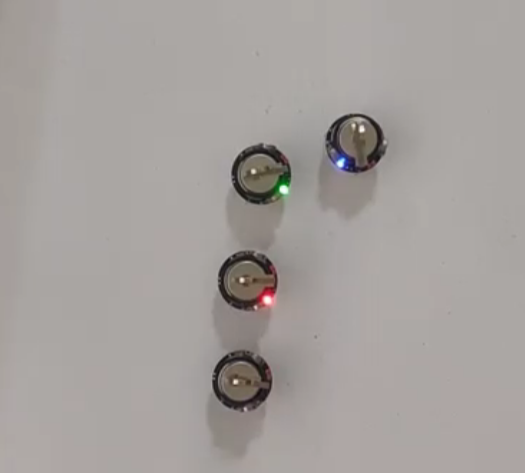
\includegraphics[width=4in]{gradient-edgefollowing.png}}
	\caption{\href{https://drive.google.com/drive/folders/14PzarH4uEqTsYBiknOU7pAX3xXhWmLxa/view}{Gradient formation and Edge following integration with TOTAL\_NUM\_COMMUNICATION\_GRADIENT=20 and TOTAL\_NUM\_COMMUNICATION = 15}}
	\label{fig:Gradient formation and Edge following integration}
\end{figure}

\chapter{Future scope}
By doing gradient formation and edge following, we are bringing robots in a group near reference robot one by one.
So scope for next work is to guide the robot which has come near reference robot to form predefined shape.
\newline Challenges for shape formation extending the same codes are as follows:
\begin{enumerate}
    \item We are using single reference robot for gradient formation. But when we want to guide a robot to a position in predefined shape, we will need minimum 2-3 reference robots.
    \item On laboratory scale we can hardcore the reference robot and extend the same code. But on large scale we will require more complex algorithms.
    \item For our experiment, we have kept the robots in straight line initially. So it is easy to identify outermost robot and make it orbit. In case of randomly placed robots, we will require to add few more parameters in the code.
    \item Then we can use the same code done by our previous batch and form some shape.
\end{enumerate}

\chapter{Acknowledgment}
We would like to thank Anurag Gupta for his teaching assistance and  clearing our silliest doubts. We would like to thanks lab staff for maintaining a healthy number of working robots. We would also like to thank Prof. Leena Vachhani and Prof. Arpita Sinha for all the support and guidance. We thank Adwiath Vijaykumar for coordination of lab report work and cooperation.

\appendix
\chapter{Code for star robot}
\lstinputlisting{code/orbit_star.c}
\label{orbit_star.c}
\lstset{
	language=C,
	numbers=left,
	stepnumber=1,
	numbersep=5pt,
	backgroundcolor=\color{white},
	showspaces=false,
	showstringspaces=false,
	showtabs=false,       
	tabsize=2,           
	captionpos=b,                   
	breaklines=true,               
https://www.overleaf.com/project/5e568db9629d1c00017eba88	breakatwhitespace=true,       
	basicstyle=\ttfamily,
	keywordstyle=\color{blue}\ttfamily,
	stringstyle=\color{red}\ttfamily,
	commentstyle=\color{ForestGreen}\ttfamily,
	%identifierstyle=\color{Mulberry},
	morecomment=[l][\color{BrickRed}]{\#},
	numberstyle=\color{gray}
}

\chapter{Code for planet robot}
\lstinputlisting{code/orbit_planet.c}
\label{orbit_planet.c}
\lstset{
	language=C,
	numbers=left,
	stepnumber=1,
	numbersep=5pt,
	backgroundcolor=\color{white},
	showspaces=false,
	showstringspaces=false,
	showtabs=false,       
	tabsize=2,           
	captionpos=b,                   
	breaklines=true,               
	breakatwhitespace=true,       
	basicstyle=\ttfamily,
	keywordstyle=\color{blue}\ttfamily,
	stringstyle=\color{red}\ttfamily,
	commentstyle=\color{ForestGreen}\ttfamily,
	%identifierstyle=\color{Mulberry},
	morecomment=[l][\color{BrickRed}]{\#},
	numberstyle=\color{gray}
}

\chapter{Code for planet robot with multiple stars}
\lstinputlisting{code/orbit_planet_ms.c}
\label{orbit_planet_ms.c}
\lstset{
	language=C,
	numbers=left,
	stepnumber=1,
	numbersep=5pt,
	backgroundcolor=\color{white},
	showspaces=false,
	showstringspaces=false,
	showtabs=false,       
	tabsize=2,           
	captionpos=b,                   
	breaklines=true,               
	breakatwhitespace=true,       
	basicstyle=\ttfamily,
	keywordstyle=\color{blue}\ttfamily,
	stringstyle=\color{red}\ttfamily,
	commentstyle=\color{ForestGreen}\ttfamily,
	%identifierstyle=\color{Mulberry},
	morecomment=[l][\color{BrickRed}]{\#},
	numberstyle=\color{gray}
}

\chapter{Code for reference robot}
\lstinputlisting{code/ref-bot.c}
\label{ref-bot.c}
\lstset{
	language=C,
	numbers=left,
	stepnumber=1,
	numbersep=5pt,
	backgroundcolor=\color{white},
	showspaces=false,
	showstringspaces=false,
	showtabs=false,       
	tabsize=2,           
	captionpos=b,                   
	breaklines=true,               
	breakatwhitespace=true,       
	basicstyle=\ttfamily,
	keywordstyle=\color{blue}\ttfamily,
	stringstyle=\color{red}\ttfamily,
	commentstyle=\color{ForestGreen}\ttfamily,
	%identifierstyle=\color{Mulberry},
	morecomment=[l][\color{BrickRed}]{\#},
	numberstyle=\color{gray}
}

\chapter{Code for gradient formation}
\lstinputlisting{code/gradient.c}
\label{gradient.c}
\lstset{
	language=C,
	numbers=left,
	stepnumber=1,
	numbersep=5pt,
	backgroundcolor=\color{white},
	showspaces=false,
	showstringspaces=false,
	showtabs=false,       
	tabsize=2,           
	captionpos=b,                   
	breaklines=true,               
	breakatwhitespace=true,       
	basicstyle=\ttfamily,
	keywordstyle=\color{blue}\ttfamily,
	stringstyle=\color{red}\ttfamily,
	commentstyle=\color{ForestGreen}\ttfamily,
	%identifierstyle=\color{Mulberry},
	morecomment=[l][\color{BrickRed}]{\#},
	numberstyle=\color{gray}
}

\chapter{Code for edge following}
\lstinputlisting{code/edge-following.c}
\label{edge-following.c}
\lstset{
	language=C,
	numbers=left,
	stepnumber=1,
	numbersep=5pt,
	backgroundcolor=\color{white},
	showspaces=false,
	showstringspaces=false,
	showtabs=false,       
	tabsize=2,           
	captionpos=b,                   
	breaklines=true,               
	breakatwhitespace=true,       
	basicstyle=\ttfamily,
	keywordstyle=\color{blue}\ttfamily,
	stringstyle=\color{red}\ttfamily,
	commentstyle=\color{ForestGreen}\ttfamily,
	%identifierstyle=\color{Mulberry},
	morecomment=[l][\color{BrickRed}]{\#},
	numberstyle=\color{gray}
}

\chapter{Code for gradient formation and edge following integration}
\lstinputlisting{code/int-grad-edgefollow.c}
\label{int-grad-edgefollow.c}
\lstset{
	language=C,
	numbers=left,
	stepnumber=1,
	numbersep=5pt,
	backgroundcolor=\color{white},
	showspaces=false,
	showstringspaces=false,
	showtabs=false,       
	tabsize=2,           
	captionpos=b,                   
	breaklines=true,               
	breakatwhitespace=true,       
	basicstyle=\ttfamily,
	keywordstyle=\color{blue}\ttfamily,
	stringstyle=\color{red}\ttfamily,
	commentstyle=\color{ForestGreen}\ttfamily,
	%identifierstyle=\color{Mulberry},
	morecomment=[l][\color{BrickRed}]{\#},
	numberstyle=\color{gray}
}
\end{document}
